% ============================================================
% Kapitola 4 — Výsledky a diskuse  (DISCOUNT = 0 %, METRIKA = EAA)
% ============================================================
\chapter{Výsledky a~diskuse}
\label{chap:vysledky}

V~této kapitole prezentujeme výsledky stochastické Monte Carlo simulace
modelu navrženého v~kapitole~\ref{chap:metodologie} se~zaměřením
na~\emph{rizikový profil} pěstování \textit{Miscanthus~$\times$~giganteus}
a~rychle rostoucích dřevin (SRC vrba) v~podmínkách České republiky.
V~souladu se~zadáním práce jsou~rizikové ukazatele jádrem analýzy;
ekonomické metriky slouží pouze jako rámec, ve~kterém se~rizikový profil
projevuje.

\section{Konfigurace baseline}
\label{sec:vysledky-baseline-konfig}

\begin{table}[H]
\centering
\caption{Konfigurace baseline scénáře pro~kapitolu~\ref{chap:vysledky}.}
\label{tab:baseline-config}
\renewcommand{\arraystretch}{1.2}
\begin{tabular}{ll}
\toprule
\textbf{Parametr} & \textbf{Hodnota} \\
\midrule
Klimatická zóna & Střední Evropa / Mírné pásmo \\
Plocha plantáže & 10~ha \\
Počet Monte Carlo scénářů $N$ & 10\,000 \\
Diskontní sazba $r$ & 0~\% \\
Dotační podíl na~CAPEX & 0~\% \\
Pachtovné (varianta s~nájmem) & 200~EUR/ha/rok \\
Korelace $\rho$ (počasí $\leftrightarrow$ cena) & 0 \\
Dekarbonizační drift $g$ & 1~\%/rok \\
Eskalace provozních nákladů $e_o$ & 2~\%/rok \\
Pravděpodobnost klimatického stresu $p_w$ & 5~\% \\
Pravděpodobnost selhání plantáže $p_f$ & 5~\% \\
Životnost Miscanthus / SRC vrba & 26~/~30~let \\
Výchozí prodejní cena Miscanthus / SRC & 117~/~130~EUR/t~DM \\
\bottomrule
\end{tabular}
\end{table}

\paragraph{Volba diskontní sazby $r = 0$~\%.}
Akademická volba diskontní sazby pro~víceleté energetické plodiny v~ČR
se~v~literatuře pohybuje v~širokém pásmu $5$--$11{,}5~\%$
\citep{knapek_2024,Janota2023}. Cílem této práce je~však \emph{ohodnocení
rizika}, nikoli predikce realistické úrovně budoucí ziskovosti, a~konkrétní
hodnota $r$ je~jednou z~klíčových nejistot ekonomického modelu, kterou
nelze empiricky ověřit. V~baseline scénáři volíme proto \emph{nulový
diskont}, což eliminuje arbitrární vliv $r$ na~výsledné rozdělení
a~činí výsledky závislé pouze na~modelovaných stochastických jevech
(počasí, cena, selhání plantáže).

\paragraph{Volba EAA jako primární ekonomické metriky.}
Vzhledem k~tomu, že~Miscanthus má~životnost \mbox{26 let} a~SRC vrba
\mbox{30 let}, není přímé srovnání NPV obou plodin metodicky korektní ---
delší životnost přirozeně akumuluje vyšší NPV, aniž by~to~vypovídalo
o~efektivnější investici. Pro~zachování srovnatelnosti používáme
\textbf{ekvivalentní roční anuitu (EAA)}, definovanou v~sekci~\ref{sec:eaa_theory},
která převádí celkové NPV na~ročně přepočtenou hodnotu. Při $r = 0$~\%
se~vztah zjednodušuje na~$\mathrm{EAA} = \mathrm{NPV} / n$, tedy
průměrný roční cash flow přes celou životnost projektu. EAA tak~vyjadřuje,
kolik EUR \emph{v~průměru za~rok} plantáž vydělá nebo prodělá ---
hodnota přímo srovnatelná napříč plodinami i~kategoriemi půdy.

\paragraph{Sledované rizikové ukazatele.}
\begin{itemize}
    \item \textbf{$P(\mathrm{EAA} > 0)$} --- pravděpodobnost ziskovosti
          investice (klíčový ukazatel pro~rozhodování pěstitele).
    \item \textbf{VaR$_{5\%}$} --- 5.~percentil rozdělení EAA
          (nejhorší roční výsledek s~95\% spolehlivostí).
    \item \textbf{CVaR$_{5\%}$} --- průměrná hloubka chvostové ztráty
          v~dolních $5~\%$ scénářů.
    \item \textbf{$\sigma_{\mathrm{CF}}^{\mathrm{rok}}$} --- směrodatná
          odchylka ročního cash flow; reflektuje \emph{likviditní
          riziko} pěstitele.
    \item \textbf{Pravděpodobnost a~průměrná doba návratnosti}.
\end{itemize}

\paragraph{Kritická poznámka k~prodejní ceně.}
Výchozí prodejní cena $117$~EUR/t~DM (Miscanthus) a~$130$~EUR/t~DM
(SRC vrba) je~v~modelu nastavena jako \emph{horní mez kvalifikovaného
expertního odhadu}, odvozená bottom-up z~oficiální referenční ceny
biomasy kategorie~1 dle~\citet{Vyhlaska315_2025} (190~K\v{c}/GJ;
viz~§~\ref{sec:cena_pref}). Reálná tržní cena, za~kterou je~biomasa
v~ČR vykupována, je~v~praxi předmětem bilaterálních smluv mezi pěstitelem
a~teplárnou; její konkrétní úroveň ovlivňují kvalitativní parametry
biomasy, vyjednávací pozice stran a~struktura dotačního rámce na~straně
odběratele --- faktory, které tato práce nemodeluje. Absolutní hodnoty
EAA v~následujících sekcích je~tedy nutno chápat jako \emph{horní mez
ziskového potenciálu}; \textbf{relativní rizikový profil obou plodin
a~jejich vzájemné srovnání zůstávají nezávislé na~konkrétní úrovni ceny}.
Cílem této kapitoly je proto kvantifikovat, \textit{jak} se~mění riziko
napříč kvalitami půdy a~plodinami, nikoli \textit{kolik} přesně pěstitel
vydělá.

\paragraph{Struktura analýzy.}
Analýza je~organizována \emph{soil-first} přístupem od~nejhorší k~nejlepší
půdě. V~každé sekci porovnáváme obě plodiny s~důrazem na~rizikové ukazatele.

% ============================================================
\section{Nevhodná půda (Miscanthus 0--4 / SRC 0--4 t DM/ha/rok)}
\label{sec:vysledky-nevhodna}

Nevhodnou kategorii uvádíme \emph{pouze pro~úplnost} --- představuje
stanoviště, na~kterých by~žádný racionální pěstitel energetické plodiny
nezakládal. Maximální peakový výnos $0$--$4$~t~DM/ha/rok znamená, že~ani
v~nejlepším roce plantáž nedosáhne výnosů typických pro~marginální
zemědělskou produkci, natož aby~pokryla investiční náklady.

\begin{figure}[H]
\centering

\includegraphics[width=0.95\textwidth]{img/kap04/04_nevhodna_eaa_distribuce.pdf}
\caption{Distribuce ekvivalentní roční anuity (EAA) pro~Nevhodnou půdu
($N = 10\,000$, diskont 0~\%). Obě distribuce leží plně v~záporné
polorovině; pravděpodobnost ziskovosti je~nulová pro~obě plodiny.}
\label{fig:nevhodna-eaa}
\end{figure}

\begin{table}[H]
\centering
\caption{Rizikové ukazatele pro~Nevhodnou půdu (EAA v~EUR/rok pro~10~ha plantáž).}
\label{tab:nevhodna-metriky}
\renewcommand{\arraystretch}{1.15}
\begin{tabular}{lrr}
\toprule
\textbf{Ukazatel} & \textbf{Miscanthus} & \textbf{SRC vrba} \\
\midrule
$P(\mathrm{EAA} > 0)$                     & $0{,}0~\%$ & $0{,}0~\%$ \\
Mean EAA (EUR/rok)                        & $-3\,667$  & $-2\,547$ \\
VaR$_{5\%}$ EAA (EUR/rok)                 & $-4\,614$  & $-3\,243$ \\
CVaR$_{5\%}$ EAA (EUR/rok)                & $-4\,782$  & $-3\,350$ \\
$\sigma_{\mathrm{CF}}^{\mathrm{rok}}$ (EUR/rok) & $5\,440$ & $3\,072$ \\
Pravděpodobnost návratnosti               & $0{,}0~\%$ & $0{,}0~\%$ \\
\bottomrule
\end{tabular}
\end{table}

Žádný z~$10\,000$ simulovaných scénářů se~u~obou plodin nedostane
k~návratnosti počáteční investice; investice je~tedy \emph{deterministicky
ztrátová}. Nižší absolutní ztráta u~SRC vrby (mean EAA $-2\,547$~vs.~$-3\,667$
EUR/rok) reflektuje strukturálně nižší investiční náklad RRD (CAPEX
$1\,509$~vs.~$3\,045$~EUR/ha pro~Miscanthus). \textbf{Závěr:}
\emph{stanoviště této kategorie nejsou ekonomicky způsobilá pro~komerční
pěstování energetické biomasy} a~v~následujících analýzách je~uvádíme
pouze pro~úplnost.


% ============================================================
\section{Neúrodná půda (Miscanthus 4--7 / SRC 4--7 t DM/ha/rok)}
\label{sec:vysledky-neurodna}

Neúrodná kategorie zahrnuje stanoviště s~peakovým výnosem $4$--$7$~t~DM/ha/rok
(lehké písčité půdy, plochy s~omezeným zásobováním vodou, podhorské
lokality).

\begin{figure}[H]
\centering

\includegraphics[width=0.95\textwidth]{img/kap04/04_neurodna_eaa_distribuce.pdf}
\caption{Distribuce EAA pro~Neúrodnou půdu. Distribuce obou plodin
leží převážně v~záporné polorovině s~pouze marginálním dosahem
do~ziskové zóny u~SRC vrby.}
\label{fig:neurodna-eaa}
\end{figure}

\begin{table}[H]
\centering
\caption{Rizikové ukazatele pro~Neúrodnou půdu (EAA v~EUR/rok pro~10~ha plantáž).}
\label{tab:neurodna-metriky}
\renewcommand{\arraystretch}{1.15}
\begin{tabular}{lrr}
\toprule
\textbf{Ukazatel} & \textbf{Miscanthus} & \textbf{SRC vrba} \\
\midrule
$P(\mathrm{EAA} > 0)$                     & $0{,}1~\%$ & $1{,}8~\%$ \\
Mean EAA (EUR/rok)                        & $-1\,903$  & $-993$ \\
VaR$_{5\%}$ EAA (EUR/rok)                 & $-2\,812$  & $-1\,709$ \\
CVaR$_{5\%}$ EAA (EUR/rok)                & $-3\,028$  & $-1\,863$ \\
$\sigma_{\mathrm{CF}}^{\mathrm{rok}}$ (EUR/rok) & $6\,029$ & $5\,416$ \\
Pravděpodobnost návratnosti               & $1{,}0~\%$ & $16{,}9~\%$ \\
Průměrná doba návratnosti (let)           & $14{,}0$   & $18{,}3$ \\
\bottomrule
\end{tabular}
\end{table}

\subsection*{Diskuse rizikového profilu}

Posun do~vyšší výnosové kategorie $4$--$7$~t~DM/ha/rok přibližuje obě
plodiny směrem k~ekonomické přijatelnosti, ale~obě varianty zůstávají
\emph{prakticky vždy ztrátové} ($P(\mathrm{EAA}>0) \leq 1{,}8~\%$).
Klíčovým rizikovým rozdílem mezi plodinami je~zde
\textbf{pravděpodobnost kumulativní návratnosti}: zatímco Miscanthus
ji~dosahuje pouze v~$1~\%$ scénářů, SRC vrba dosahuje
\textbf{$16{,}9~\%$} při průměrné době $18{,}3$~let.

Tento rozdíl ilustruje strukturální výhodu RRD: nižší investiční náklad
umožňuje, aby~se~plantáž v~určitém pásmu scénářů --- typicky těch
s~kombinací příznivého počasí a~horní úrovně peakového výnosu --- dostala
alespoň na~kumulativní break-even. Hodnota
$\mathrm{CVaR}_{5\%}^{(S)} = -1\,863$~EUR/rok (oproti
$-3\,028$~EUR/rok u~Miscanthusu) odráží stejný mechanismus na~chvostu
distribuce: i~ve~scénářích s~nejnepříznivějším průběhem ztrácí pěstitel
SRC vrby o~přibližně $1\,200$~EUR za~rok méně.

\textbf{Závěr:} Neúrodná půda představuje hraniční zónu, ve~které je~Miscanthus
prakticky vždy ztrátový. SRC vrba v~malém procentu scénářů dosahuje
kumulativní návratnosti, ale~bez dotační podpory zde nelze pěstování
doporučit. Energetické plodiny v~tomto pásmu mají smysl pouze
v~kombinaci s~dotační podporou nebo na~půdě bez alternativního využití.


% ============================================================
\section{Průměrná půda (Miscanthus 7--14 / SRC 7--12 t DM/ha/rok)}
\label{sec:vysledky-prumerna}

Průměrná kategorie reprezentuje typickou českou ornou půdu střední
bonity, která tvoří dominantní část výměry zemědělského půdního fondu
ČR. Peakový výnos dosahuje $7$--$14$~t~DM/ha/rok (Miscanthus)
a~$7$--$12$~t~DM/ha/rok (SRC vrba).

\begin{figure}[H]
\centering

\includegraphics[width=0.95\textwidth]{img/kap04/04_prumerna_eaa_distribuce.pdf}
\caption{Distribuce EAA pro~Průměrnou půdu. Distribuce obou plodin
přechází přes nulovou hranici; SRC vrba leží převážně v~kladné
polorovině, Miscanthus je~symetrický kolem nuly.}
\label{fig:prumerna-eaa}
\end{figure}

\begin{table}[H]
\centering
\caption{Rizikové ukazatele pro~Průměrnou půdu (EAA v~EUR/rok pro~10~ha plantáž).}
\label{tab:prumerna-metriky}
\renewcommand{\arraystretch}{1.15}
\begin{tabular}{lrr}
\toprule
\textbf{Ukazatel} & \textbf{Miscanthus} & \textbf{SRC vrba} \\
\midrule
$P(\mathrm{EAA} > 0)$                     & $68{,}3~\%$ & $93{,}3~\%$ \\
Mean EAA (EUR/rok)                        & $+621$      & $+1\,363$ \\
VaR$_{5\%}$ EAA (EUR/rok)                 & $-1\,302$   & $-156$ \\
CVaR$_{5\%}$ EAA (EUR/rok)                & $-1\,601$   & $-535$ \\
$\sigma_{\mathrm{CF}}^{\mathrm{rok}}$ (EUR/rok) & $7\,128$ & $9\,150$ \\
Pravděpodobnost návratnosti               & $76{,}2~\%$ & $96{,}1~\%$ \\
Průměrná doba návratnosti (let)           & $11{,}4$    & $13{,}3$ \\
\bottomrule
\end{tabular}
\end{table}

\subsection*{Diskuse rizikového profilu}

Průměrná půda je~\textbf{klíčovým bodem ekonomické a~rizikové analýzy},
neboť tvoří dominantní výměru zemědělského fondu ČR. Distribuce EAA
přechází přes nulovou hranici a~v~tomto pásmu se~poprvé v~analýze
projevují \emph{strukturální rozdíly v~rizikovém profilu obou plodin}.

\paragraph{Pravděpodobnost ziskovosti.}
Klíčový ukazatel $P(\mathrm{EAA}>0)$ ostře odlišuje obě plodiny:
SRC vrba dosahuje $93{,}3~\%$ pravděpodobnosti zisku, zatímco Miscanthus
pouze $68{,}3~\%$. Z~pohledu rozhodování pěstitele to~znamená, že~při
volbě SRC vrby selže přibližně každý 15. scénář, zatímco
u~Miscanthusu každý 3.~scénář.

\paragraph{Chvostové riziko (VaR a~CVaR).}
Hodnota VaR$_{5\%}$ EAA ukazuje, jaká je~nejhorší roční ztráta v~$95~\%$
realistických scénářů: pro~SRC vrbu je~to~$-156$~EUR/rok, zatímco
pro~Miscanthus $-1\,302$~EUR/rok. Rozdíl
$\Delta \mathrm{VaR} \approx +1\,150$~EUR/rok ve~prospěch SRC ilustruje,
že~jeho distribuce je~výrazně posunutá doprava (kompaktnější chvost ztrát).
Hodnota CVaR$_{5\%}$ EAA pak prohlubuje tento obraz: průměrná hloubka
ztráty v~nejhorších $5~\%$ scénářů je~$-535$~EUR/rok pro~SRC vrbu
oproti $-1\,601$~EUR/rok pro~Miscanthus --- chvostová ztráta SRC vrby
je~tedy přibližně třetinová.

\paragraph{Likviditní riziko (volatilita ročního CF).}
Zde dochází k~zajímavé inverzi: $\sigma_{\mathrm{CF}}^{(S)} = 9\,150$~EUR/rok
převyšuje $\sigma_{\mathrm{CF}}^{(M)} = 7\,128$~EUR/rok o~$28~\%$,
přestože SRC vrba dosahuje vyššího mean EAA i~nižšího chvostového rizika.
Tato inverze je~vysvětlitelná \emph{strukturou sklizňového cyklu}:
roční sklizeň Miscanthusu vede k~plynulému toku tržeb, zatímco tříletý
rotační cyklus SRC produkuje výrazné špičky cash flow v~roce sklizně
a~období bez příjmů v~mezilehlých letech. Volatilita ročního CF tedy
\emph{není rizikem návratnosti investice}, ale~\emph{likviditním rizikem}
pěstitele --- nutností finančního plánování přes~několikaleté horizonty
a~držet rezervu pro~roky bez sklizně.

\paragraph{Pravděpodobnost návratnosti.}
Doplňkový ukazatel pravděpodobnosti kumulativní návratnosti $96{,}1~\%$
(SRC) vs.~$76{,}2~\%$ (M) potvrzuje předchozí závěr: i~scénáře, které
nedosáhnou kladného EAA, se~u~SRC ve~většině případů alespoň dostanou
zpět k~vyrovnané kumulativní bilanci.

\textbf{Závěr:} Na~průměrné půdě je~SRC vrba investičně robustně
zisková ($P(\mathrm{EAA}>0) \approx 93~\%$, VaR$_{5\%} \approx -150$~EUR/rok),
zatímco Miscanthus představuje rizikově neutrální variantu s~vysokou
varianci výsledků ($P(\mathrm{EAA}>0) \approx 68~\%$,
VaR$_{5\%} \approx -1\,300$~EUR/rok). Volba plodiny musí zohlednit
nejen ekonomický výnos, ale~i~likviditní toleranci pěstitele, která
hraje proti SRC vrbě.


% ============================================================
\section{Optimální půda (Miscanthus 14--16 / SRC 12--15 t DM/ha/rok)}
\label{sec:vysledky-optimalni}

Optimální kategorie zahrnuje nejúrodnější zemědělské půdy v~ČR ---
černozemě, hnědozemě, kvalitní hnědé půdy nížin Polabí, jižní Moravy
a~Hané. Peakový výnos dosahuje $14$--$16$~t~DM/ha/rok (Miscanthus)
a~$12$--$15$~t~DM/ha/rok (SRC vrba), což je~v~souladu s~empirickými
hodnotami doloženými dlouhodobými polními pokusy
\citep{Janota2023, Weger2021}.

\begin{figure}[H]
\centering

\includegraphics[width=0.95\textwidth]{img/kap04/04_optimalni_eaa_distribuce.pdf}
\caption{Distribuce EAA pro~Optimální půdu. Obě distribuce leží
prakticky kompletně v~kladné polorovině; SRC vrba dosahuje vyššího mean
EAA i~výrazně nižšího chvostového rizika.}
\label{fig:optimalni-eaa}
\end{figure}

\begin{table}[H]
\centering
\caption{Rizikové ukazatele pro~Optimální půdu (EAA v~EUR/rok pro~10~ha plantáž).}
\label{tab:optimalni-metriky}
\renewcommand{\arraystretch}{1.15}
\begin{tabular}{lrr}
\toprule
\textbf{Ukazatel} & \textbf{Miscanthus} & \textbf{SRC vrba} \\
\midrule
$P(\mathrm{EAA} > 0)$                     & $97{,}6~\%$ & $97{,}5~\%$ \\
Mean EAA (EUR/rok)                        & $+2\,895$   & $+3\,319$ \\
VaR$_{5\%}$ EAA (EUR/rok)                 & $+939$      & $+1\,693$ \\
CVaR$_{5\%}$ EAA (EUR/rok)                & $-267$      & $+367$ \\
$\sigma_{\mathrm{CF}}^{\mathrm{rok}}$ (EUR/rok) & $8\,255$ & $12\,677$ \\
Pravděpodobnost návratnosti               & $97{,}6~\%$ & $97{,}5~\%$ \\
Průměrná doba návratnosti (let)           & $8{,}9$     & $10{,}3$ \\
\bottomrule
\end{tabular}
\end{table}

\subsection*{Diskuse rizikového profilu}

Optimální půda představuje scénář, ve~kterém jsou~obě plodiny
\emph{robustně investičně přijatelné} s~prakticky shodnou
pravděpodobností ziskovosti $\approx 97{,}5~\%$. \emph{Rizikový rozdíl}
se~však projevuje v~chvostových ukazatelích a~ve~struktuře cash flow.

\paragraph{Chvostové riziko --- klíčová převaha SRC.}
VaR$_{5\%}$ EAA je~kladný u~obou plodin, což znamená, že~i~v~$95~\%$
nejhorších scénářů zůstává plantáž zisková. SRC vrba má~ovšem
\textbf{strukturálně příznivější chvost}:
\begin{itemize}
    \item VaR$_{5\%}^{(S)} = +1\,693$~EUR/rok vs.~$+939$~EUR/rok
          u~Miscanthusu --- spodní 5\% scénářů SRC vrby vydělá
          ročně téměř dvojnásobek.
    \item CVaR$_{5\%}^{(S)} = +367$~EUR/rok vs.~$-267$~EUR/rok ---
          \textbf{průměrný chvostový scénář SRC vrby je~ziskový}, zatímco
          u~Miscanthusu je~mírně ztrátový.
\end{itemize}
Tato převaha SRC v~chvostové zóně pramení z~delší životnosti plantáže
(30 vs.~26~let), nižšího CAPEXu (1\,509~vs.~3\,045~EUR/ha) a~vyšší
ceny biomasy DM (130 vs.~117~EUR/t~DM, viz~§~\ref{sec:cena_kalibrace}).

\paragraph{Likviditní riziko v~optimálních podmínkách.}
Volatilita ročního cash flow zůstává vyšší u~SRC vrby
($12\,677$ vs.~$8\,255$~EUR/rok). V~optimálních podmínkách dosahují
peakové sklizně SRC vrby vysokých absolutních hodnot, čímž
\emph{zesilují} prokmitání cash flow oproti rovnoměrnému toku
Miscanthusu. Pro~pěstitele to~znamená klasický \emph{trade-off}:
\begin{quote}
\textit{Miscanthus} = stabilní roční tok tržeb, kratší doba
návratnosti ($8{,}9$~let) --- vhodný pro~pěstitele s~omezenou likviditní
rezervou. \\
\textit{SRC vrba} = vyšší celkový roční ekvivalentní výnos
a~kompaktnější rizikový chvost, ale~vyšší likviditní nárok kvůli
tříletým rotacím sklizní.
\end{quote}

\textbf{Závěr:} Volba mezi plodinami na~optimální půdě je~de facto
volbou mezi \emph{stabilitou cash flow} (Miscanthus) a~\emph{nižším
chvostovým rizikem a~vyšším ročním výnosem} (SRC vrba); pravděpodobnost
ziskovosti je~u~obou plodin srovnatelná a~vysoká.

% ============================================================
\section{Citlivostní analýza klíčových odhadovaných parametrů}
\label{sec:vysledky-citlivost}

V~předchozí podsekci jsme přiznali, že~řada vstupních parametrů modelu
(prodejní ceny biomasy, cena sadebního materiálu, sklizňové náklady,
struktura OPEX, eskalace nákladů, dekarbonizační drift, volatilita
cen) byla stanovena \emph{expertním odhadem}, nikoli empiricky
z~dlouhodobých dat. Pro~čtenáře je~proto klíčové vědět, \emph{jak
robustní} jsou závěry této kapitoly vůči odchylkám od~baseline hodnot.
Tato sekce kvantifikuje vliv devíti nejvýznamnějších odhadovaných
parametrů na~tři klíčové ukazatele:
\begin{itemize}
    \item \textbf{VaR$_{5\%}$ EAA} --- 5.~percentil rozdělení ročního
          ekvivalentu (rizikové dolní pásmo);
    \item \textbf{CVaR$_{5\%}$ EAA} --- průměrná hodnota v~5\,\% nejhorších
          scénářů (chvostové riziko);
    \item \textbf{Průměr EAA} --- referenční ekonomický ukazatel.
\end{itemize}
Toto trojí pohledové vyhodnocení reflektuje, že~v~kontextu
\emph{rizikově orientované analýzy} mají rizikové ukazatele přednost
před průměrnou hodnotou.

\paragraph{Konfigurace experimentu.}
Analýzu provádíme metodou OAT (One-At-a-Time) pro~\textbf{průměrnou
půdu} ($Y_{\max} \in [7;14]$ pro~Miscanthus, $[7;12]$ pro~SRC vrbu),
neboť představuje nejcitlivější zónu rozhodování --- v~ní obě plodiny
operují blízko hranice ziskovosti a~změna parametru zde maximálně
mění strategický závěr. Simulace probíhá s~$N = 5\,000$ Monte Carlo
scénáři pro~každý OAT bod (celkem 19 běhů: baseline $+$ 9~parametrů~$\times$~2
extrémy).

\textbf{Volba rozpětí pro~každý parametr je~motivována reálným pásmem
nejistoty}, nikoli unifikovanou perturbací. Tržní ceny biomasy lze
realisticky odhadnout v~rozsahu $\pm 20\,\%$ od~aktuální tržní hladiny;
ceny sadebního materiálu v~ČR mají~mnohem širší pásmo (literární
zdroje uvádějí pro~Miscanthus $0{,}10$ až $0{,}50$~€/oddenek), proto
je~pro~ně rozpětí absolutní. Volatilita ceny $\sigma_P$ je~modelový
parametr bez~empirické referenční hodnoty pro~ČR; volíme proto rozpětí
$\pm 50\,\%$ jako konzervativní citlivostní test.

\textbf{Důležitá poznámka k~dekarbonizačnímu driftu a~eskalaci OPEX.}
Hodnoty $\pm 5\,\%$/rok pro~drift a~eskalaci představují \emph{hraniční
makroekonomické scénáře}, nikoli očekávaný roční vývoj. V~realitě
neočekáváme, že~by~cena biomasy reálně rostla o~$5\,\%$ ročně po~celou
dobu životnosti plantáže (25--30 let) --- takový dlouhodobý drift
by~odpovídal kumulativnímu zhodnocení o~více než $300\,\%$. Stejně
tak konstantní inflace OPEX o~$5\,\%$/rok by~zdvojnásobila provozní
náklady během 14 let. Tyto extrémní hodnoty zde uvádíme proto, aby~čtenář
viděl \emph{plné pásmo nejistoty} obou makroekonomických trendů
v~současné nestabilní době (období 2022--2024 v~ČR ukázalo inflační
šoky přes~$\pm 7$~p.b./rok). \textbf{Pěstitel by~měl skutečnou trajektorii
těchto parametrů aktivně sledovat} a~v~případě signálu odchylky
od~baseline (drift $1\,\%$, OPEX $2\,\%$) přepočítat investiční rozhodnutí.

\begin{table}[H]
\centering
\caption{Rozsah perturbací pro~jednotlivé odhadované parametry.}
\label{tab:citlivost-rozsah}
\small
\renewcommand{\arraystretch}{1.15}
\begin{tabular}{ll}
\toprule
\textbf{Parametr} & \textbf{Rozsah} \\
\midrule
Prodejní cena Miscanthus               & $\pm 20\,\%$ (baseline 116~€/t~DM) \\
Prodejní cena SRC vrba                 & $\pm 20\,\%$ (baseline 128~€/t~DM) \\
Cena oddenku Miscanthus                & $0{,}10$--$0{,}50$~€/ks (baseline $0{,}30$) \\
Cena řízku SRC vrba                    & $0{,}04$--$0{,}20$~€/ks (baseline $0{,}12$) \\
Sklizňové náklady                      & $\pm 20\,\%$ \\
Roční údržba (OPEX)                    & $\pm 20\,\%$ \\
Volatilita cen $\sigma_P$              & $\pm 50\,\%$ \\
Eskalace OPEX                          & $-5\,\%$ až $+5\,\%$ (baseline $+2\,\%$) \\
Dekarbonizační drift                   & $-5\,\%$ až $+5\,\%$ (baseline $+1\,\%$) \\
\bottomrule
\end{tabular}
\end{table}

\begin{figure}[H]
\centering
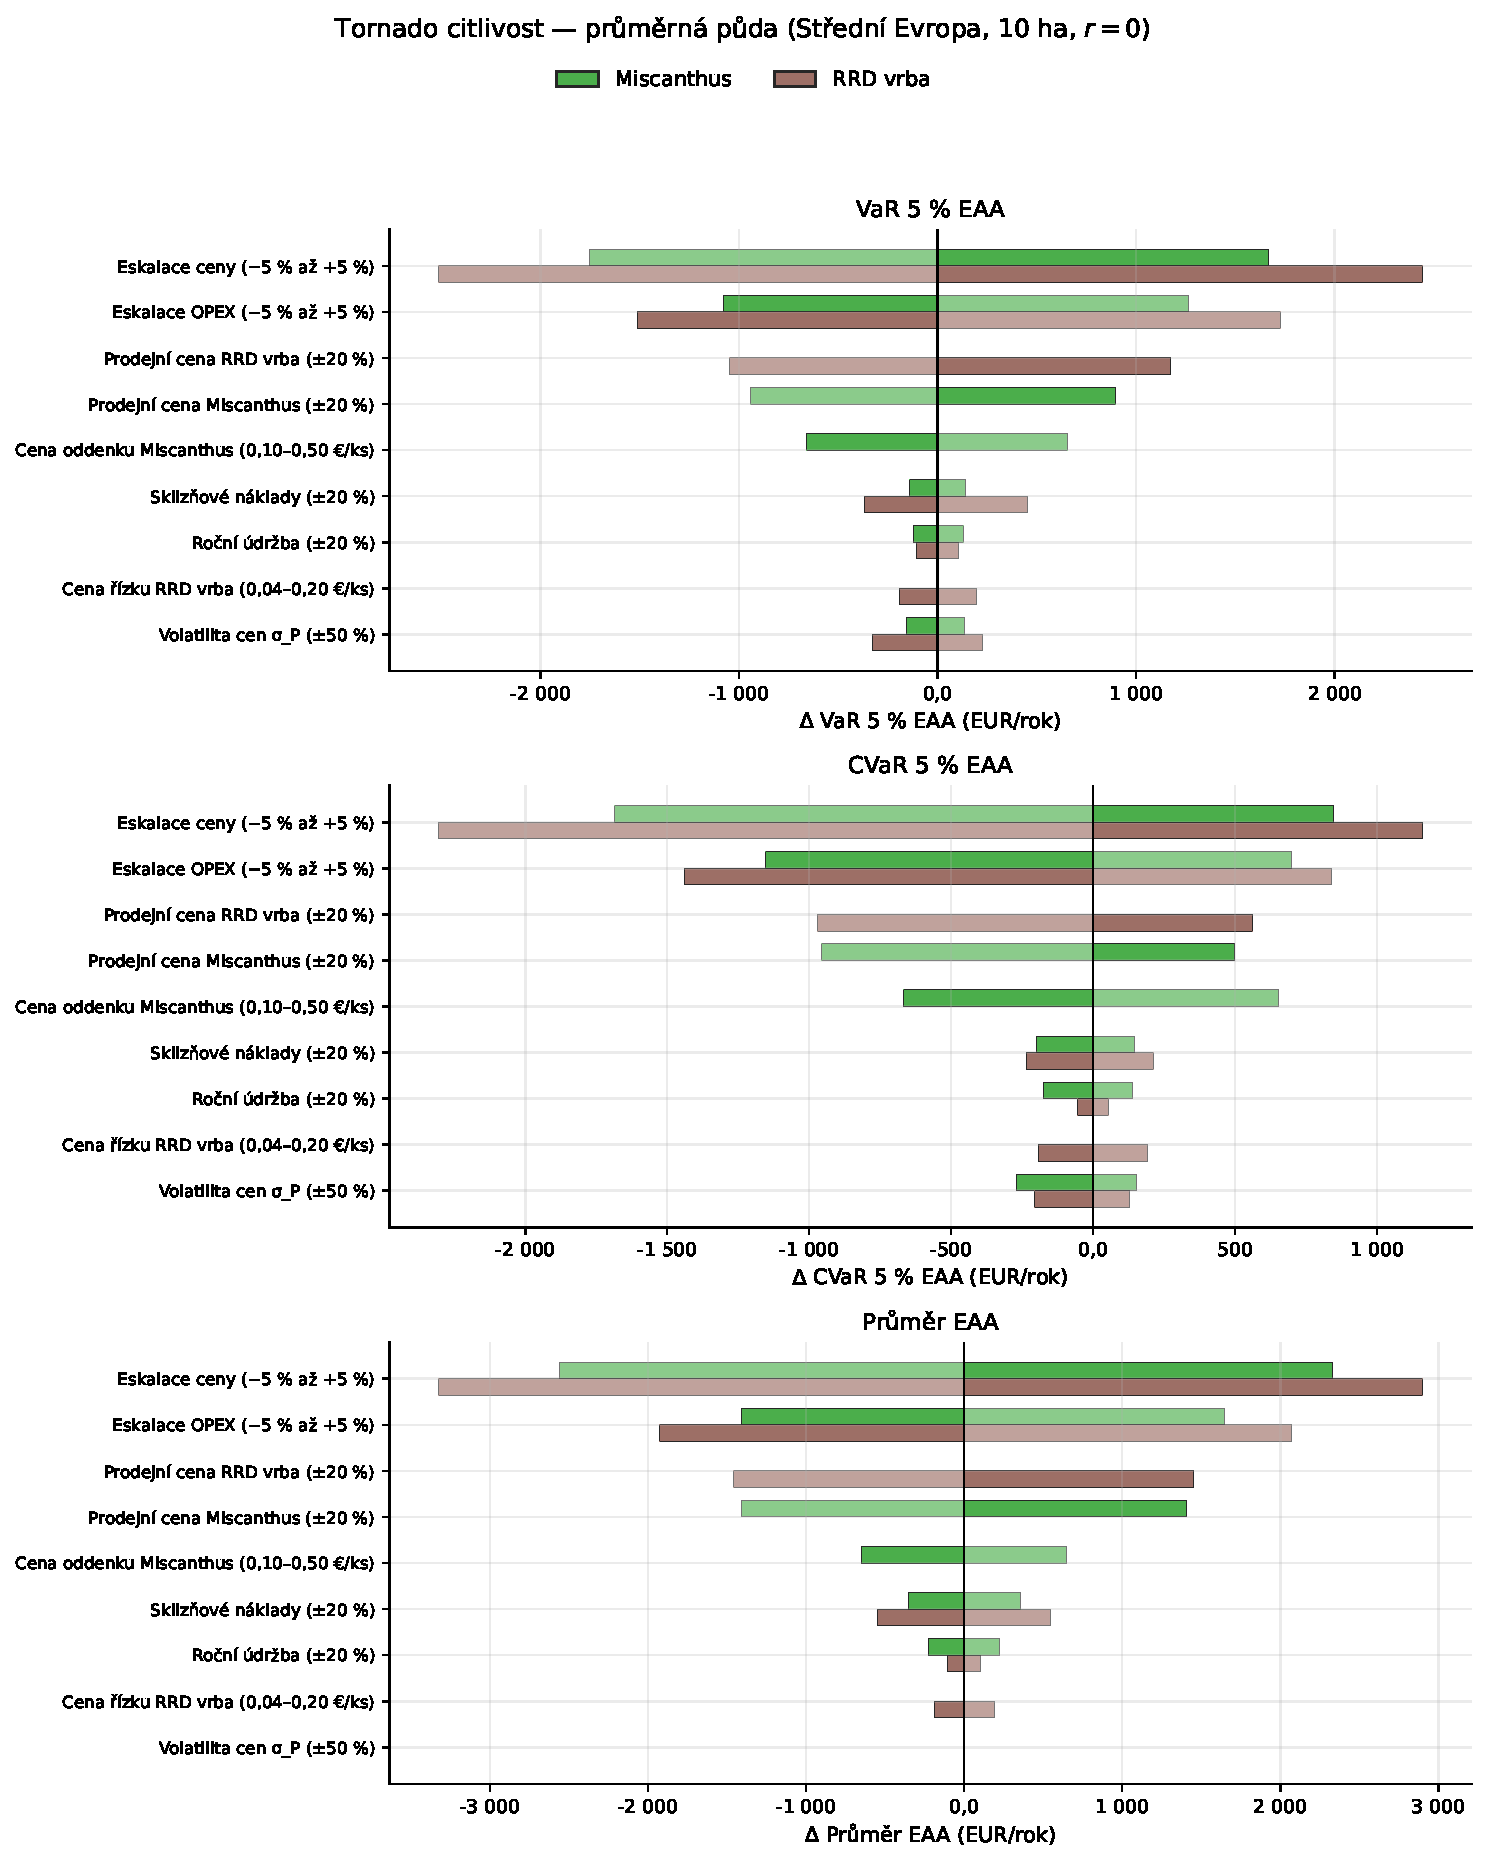
\includegraphics[width=\textwidth]{img/kap04/04_tornado_citlivost.pdf}
\caption{Tornado diagram citlivosti tří klíčových ukazatelů na~devět
odhadovaných parametrů. Levý panel = VaR$_{5\%}$ EAA (riziko), prostřední
= CVaR$_{5\%}$ EAA (chvostové riziko), pravý = průměr EAA (ekonomický
benchmark). Zelené pruhy = Miscanthus, hnědé pruhy = SRC vrba. Pruhy
řazené sestupně dle absolutní velikosti vlivu pro~Miscanthus; nejcitlivější
parametry jsou nahoře.}
\label{fig:vysledky-tornado-citlivost}
\end{figure}

\paragraph{Pořadí citlivosti pro~rizikové ukazatele (VaR a~CVaR).}
Z~levého a~prostředního panelu tornado diagramu vyplývá, že~rizikové
ukazatele reagují citlivěji a~širší škálou parametrů než průměr EAA:
\begin{enumerate}
    \item \textbf{Dekarbonizační drift dominuje VaR i~CVaR.} Posun driftu
          z~baseline $+1\,\%$ na~$-5\,\%$ propadá VaR Miscanthusu o~$-1\,752$~€/rok
          (SRC dokonce $-2\,510$~€/rok); naopak posun na~$+5\,\%$ generuje
          přírůstek až $+1\,664$~€/rok (M)~/~$+2\,440$~€/rok (S). \emph{Pesimistický
          scénář budoucího vývoje cen biomasy tedy plně eliminuje atraktivitu
          investice nezávisle na~plodině.}
    \item \textbf{Prodejní cena biomasy je~druhým nejvýznamnějším parametrem.}
          $\pm 20\,\%$ změna posune VaR o~přibližně $\pm 1\,000$~€/rok
          a~CVaR o~$\pm 600$--$1\,000$~€/rok. Vyjednávací pozice pěstitele
          tedy přímo formuje jeho rizikovou expozici.
    \item \textbf{Eskalace OPEX má~asymetrický vliv:} při~baseline
          $2\,\%$/rok je~spodní hranice $-5\,\%$ pouze hypotetická
          (deflační scénář), zatímco horní $+5\,\%$ odpovídá období
          vysoké inflace 2022--2023. Tento směr ubírá VaR M o~$-1\,078$~€/rok
          (SRC $-1\,511$); SRC je~tedy citlivější na~inflační šok.
    \item \textbf{Volatilita ceny $\sigma_P$ má~zřetelný vliv na~chvost.}
          Zatímco na~průměr EAA má~$\pm 50\,\%$ změna $\sigma_P$
          \emph{prakticky nulový dopad} ($< 5$~€/rok), na~CVaR posune
          M o~$+151$/$-270$~€/rok a~SRC o~$+129$/$-205$~€/rok. \emph{Tento
          rozdíl je~pedagogicky důležitý:} potvrzuje, že~rizikové parametry
          se~projevují primárně v~chvostových ukazatelích, nikoli v~průměru
          --- \emph{citlivost na~průměr EAA tedy systematicky podceňuje
          význam volatility a~rizik.}
    \item \textbf{Cena oddenku Miscanthusu (rozsah $0{,}10$--$0{,}50$~€/ks)}
          generuje VaR M v~rozpětí $\pm 657$~€/rok. Dolní hranice
          $0{,}10$~€/ks (komerční dovoz z~EU) by~Miscanthus výrazně přiblížila
          rentabilitě SRC; horní $0{,}50$~€/ks naopak zhoršuje jeho
          ekonomický profil dále.
\end{enumerate}

\paragraph{Klíčové zjištění pro~průměr EAA.}
Pravý panel (průměr EAA) odhaluje pořadí citlivosti, které je~částečně
odlišné:
\begin{itemize}
    \item Drift dominuje s~rozsahem $-2\,560$ až $+2\,333$~€/rok (M)
          a~$-3\,323$ až $+2\,897$~€/rok (S);
    \item následuje eskalace OPEX ($\pm 1\,500$--$2\,000$~€/rok);
    \item prodejní cena ($\pm 1\,400$~€/rok M, $\pm 1\,450$~€/rok S);
    \item cena oddenku/řízku ($\pm 650$~€/rok M, $\pm 190$~€/rok S);
    \item sklizeň ($\pm 350$--$550$), údržba ($\pm 100$--$226$);
    \item $\sigma_P$ na~průměr nemá vliv.
\end{itemize}

\paragraph{Implikace pro~důvěryhodnost závěrů.}
Tornado analýza potvrzuje, že~hlavní strukturální závěr této kapitoly
--- \emph{SRC vrba dominuje na~všech kvalitách půdy díky CAPEXové
asymetrii a~mírně vyšší prodejní ceně} --- je~\textbf{robustní vůči
většině odhadovaných parametrů s~výjimkou makroekonomických trendů
(drift, eskalace OPEX) a~vlastní prodejní ceny Miscanthusu}. Pokud
by~budoucí vývoj nepřinesl očekávaný dekarbonizační prémium
nebo~přinesl vysokou inflaci OPEX, obě plodiny by~se~mohly v~průměru
dostat do~ztráty i~na~průměrné půdě --- relativní převaha SRC by~ovšem
zůstala zachována, neboť většina parametrů má~na~SRC \emph{absolutně
větší vliv}, ale~startuje z~vyšší baseline rentability.

Pro~praktického pěstitele plyne z~tornado analýzy konkrétní strategie
řízení rizika:
\begin{enumerate}
    \item \emph{Prioritizovat dlouhodobou kupní smlouvu} ke~stabilizaci
          prodejní ceny --- největší pákový efekt napříč všemi ukazateli;
    \item \emph{Sledovat vývoj inflace OPEX} --- v~období vysoké inflace
          zvážit přechod k~plodině s~nižší absolutní citlivostí
          (Miscanthus má~kratší životnost a~tedy menší kumulativní
          dopad eskalace);
    \item \emph{Případné dotace cílit na~CAPEX} --- snížení ceny oddenku
          z~$0{,}30$ na~$0{,}10$~€/ks (např.~hromadným dovozem) přidává
          Miscanthusu $\sim 650$~€/rok, čímž se~jeho profil přibližuje
          SRC vrbě.
\end{enumerate}

Toto zjištění je~v~souladu s~výsledky paralelní studie \citet{knapek_2024},
která~identifikuje produkční cenu biomasy a~kapitálové náklady jako
klíčové veličiny rozhodující o~ekonomické životaschopnosti energetických
plodin v~ČR.

% ============================================================
\section{Vliv diskontní sazby na~rizikový profil}
\label{sec:vysledky-diskont}

Diskontní sazba $r$ je~v~ekonomické literatuře \emph{kapitola sama
o~sobě} a~její volba zásadně ovlivňuje výslednou hodnotu NPV a~tím
i~doporučení ohledně investičního rozhodnutí. V~baseline simulacích
této práce jsme záměrně volili $r = 0\,\%$ (viz~argumentace v~sekci
\ref{sec:vysledky-baseline-konfig}). \emph{Cílem této práce není
určit „správnou" diskontní sazbu pro~biomasové plantáže v~ČR};
naším primárním zaměřením je~analýza \emph{rizikového profilu}
samotného. V~budoucnu by~právě na~základě naší rizikové analýzy
mohlo být možné odvodit diskont \emph{endogenně} --- například
z~rozdělení vnitřního výnosového procenta (IRR) napříč Monte Carlo
scénáři. Nyní však tento krok ještě explicitně nečiníme.

V~této sekci proto pouze \emph{ověřujeme}, jak silně by~volba diskontu
ovlivnila rizikové ukazatele (VaR$_{5\%}$, CVaR$_{5\%}$) i~průměrnou
EAA, kdyby pěstitel přijal libovolnou nenulovou sazbu. Ukazujeme,
že~i~mírné zvýšení $r$ má~zásadní vliv \emph{nejen na~průměr,
ale~zejména na~chvostové riziko} --- proto je~budoucí pečlivá kalibrace
$r$ pro~tento typ projektu nezbytná.

\paragraph{Vliv $r$ na~rizikové ukazatele a~průměr EAA.}
Obrázek~\ref{fig:vysledky-diskont-vliv} ukazuje pro~průměrnou půdu
průběh tří klíčových ukazatelů (Průměr EAA, VaR$_{5\%}$ EAA,
CVaR$_{5\%}$ EAA) v~závislosti na~diskontní sazbě $r \in [0\,\%; 12\,\%]$.

\begin{figure}[H]
\centering
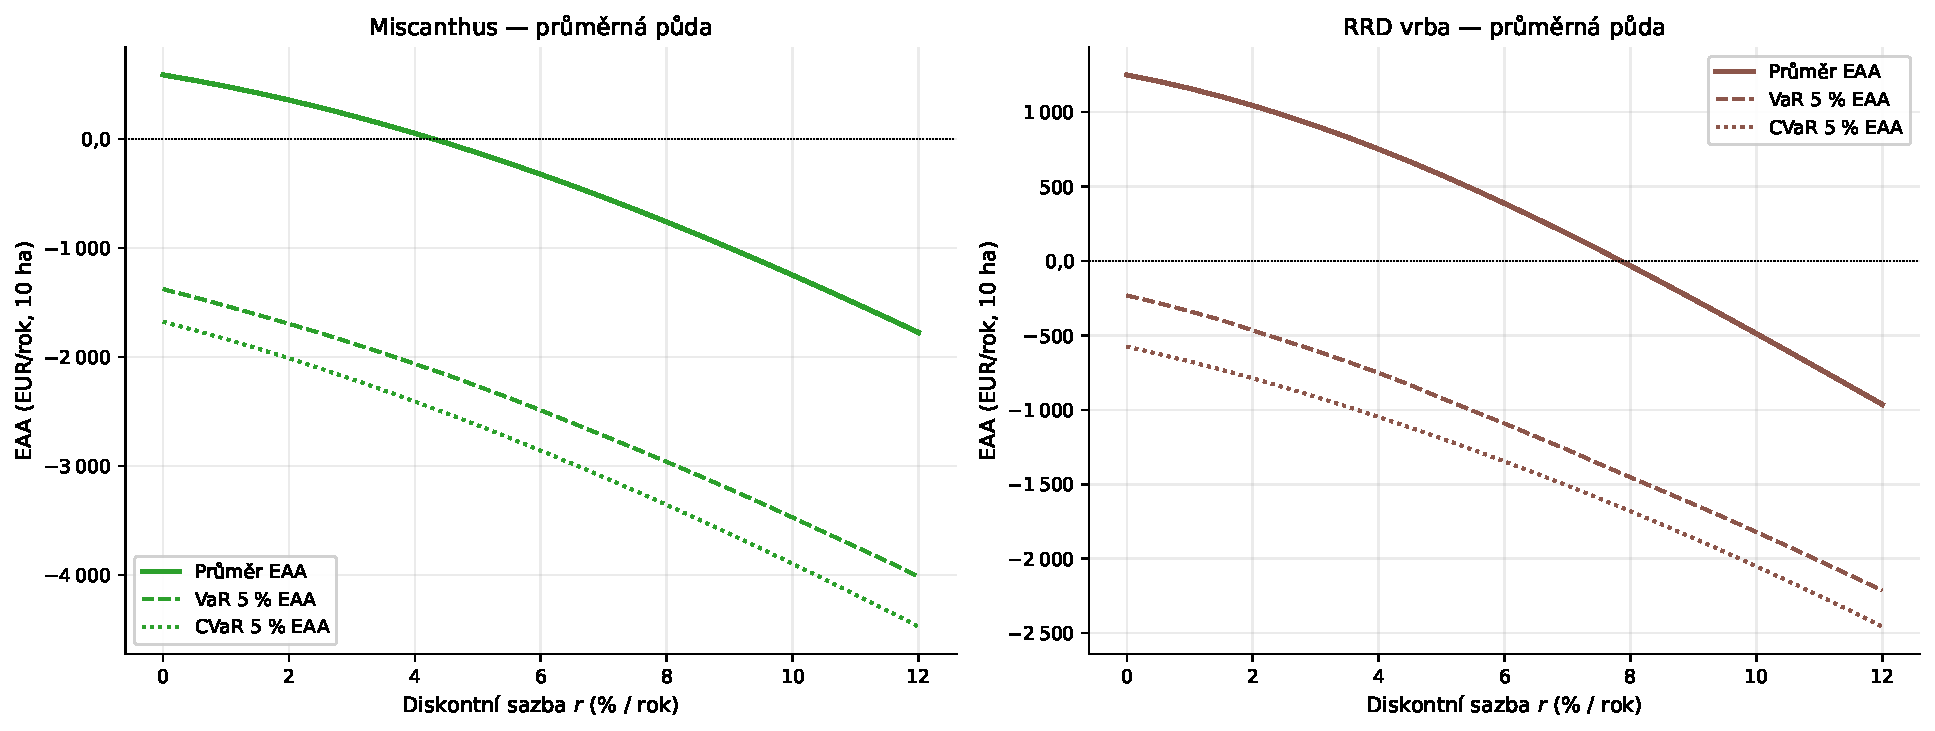
\includegraphics[width=\textwidth]{img/kap04/04_diskont_vliv.pdf}
\caption{Vliv diskontní sazby $r$ na~tři klíčové ukazatele
pro~průměrnou půdu (10~ha, $N = 10\,000$). Plná čára = průměr EAA,
čárkovaně = VaR$_{5\%}$, tečkovaně = CVaR$_{5\%}$. Levý panel Miscanthus,
pravý SRC vrba. Svislé tečkované čáry označují orientační hodnoty
$r = 3\,\%, 6\,\%, 10\,\%$.}
\label{fig:vysledky-diskont-vliv}
\end{figure}

Tabulka~\ref{tab:vysledky-diskont-body} shrnuje hodnoty pro~čtyři
referenční úrovně diskontu.

\begin{table}[H]
\centering
\caption{Hodnoty rizikových ukazatelů pro~vybrané úrovně diskontu
(průměrná půda, 10~ha).}
\label{tab:vysledky-diskont-body}
\small
\renewcommand{\arraystretch}{1.15}
\begin{tabular}{l|rrrr|rrrr}
\toprule
& \multicolumn{4}{c|}{\textbf{Miscanthus}} & \multicolumn{4}{c}{\textbf{SRC vrba}} \\
$r$  & EAA  & VaR$_5$ & CVaR$_5$ & $P_+$  & EAA  & VaR$_5$ & CVaR$_5$ & $P_+$ \\
\midrule
0 \%   & $+589$    & $-1\,377$ & $-1\,676$ & $67{,}2\,\%$ & $+1\,250$ & $-231$    & $-576$    & $92{,}1\,\%$ \\
3 \%   & $+215$    & $-1\,872$ & $-2\,203$ & $55{,}1\,\%$ & $+908$    & $-603$    & $-912$    & $85{,}2\,\%$ \\
6 \%   & $-323$    & $-2\,489$ & $-2\,859$ & $38{,}5\,\%$ & $+387$    & $-1\,092$ & $-1\,347$ & $66{,}8\,\%$ \\
10 \%  & $-1\,248$ & $-3\,473$ & $-3\,897$ & $18{,}0\,\%$ & $-488$    & $-1\,821$ & $-2\,051$ & $26{,}8\,\%$ \\
\bottomrule
\end{tabular}
\end{table}

\paragraph{Klíčová pozorování --- relativní pořadí plodin zůstává zachováno.}
Hlavní zjištění této analýzy je~zdánlivě jednoduché, ale~důležité:
\textbf{při~rostoucím diskontu klesají rizikové ukazatele obou plodin
přibližně paralelně}. Miscanthus klesá v~absolutních hodnotách o~něco
více než SRC vrba (z~$0\,\%$ na~$10\,\%$ propadne VaR M o~$\sim 2\,100$~€/rok,
SRC o~$\sim 1\,600$~€/rok), ale~tento rozdíl není dramatický, a~hlavně
\emph{nemění strukturální převahu SRC vrby}. Naopak ji~potvrzuje:
\begin{itemize}
\item Miscanthus je~rizikovější při~jakémkoli diskontu mezi $0\,\%$
      a~$12\,\%$ (jeho VaR i~CVaR leží vždy hlouběji pod nulou než u~SRC);
\item s~rostoucím diskontem se~oba ukazatele zhoršují, ale~poměr mezi
      plodinami se~zachovává;
\item naše baseline analýza (sekce~\ref{sec:vysledky-cross-soil}) tedy
      \emph{není artefaktem volby $r = 0\,\%$} --- stejné rizikové
      pořadí plodin platí napříč realistickým rozsahem diskontních sazeb.
\end{itemize}

\paragraph{Doplňkový komentář k~průměrné EAA.}
Přirozeně, s~rostoucím diskontem klesá také průměrná EAA --- budoucí
peněžní toky jsou~exponenciálně diskontovány, takže jejich přínos
k~současné hodnotě se~zmenšuje. Při~$r = 6\,\%$ se~Miscanthus dostává
do~průměrné ztráty ($-323$~€/rok), zatímco SRC vrba zůstává mírně
zisková ($+387$~€/rok); při~$r = 10\,\%$ jsou~obě plodiny ztrátové
v~průměru. Pravděpodobnost ziskovosti $P(\mathrm{NPV} > 0)$ klesá
u~Miscanthusu z~$67\,\%$ na~$18\,\%$ a~u~SRC z~$92\,\%$ na~$27\,\%$.
Tyto hodnoty potvrzují, že~\emph{volba diskontu je~klíčové investiční
rozhodnutí}, ale~zároveň nemění relativní hierarchii plodin.

\subsection{Náznak: jak by~mohl být diskont odvozen endogenně}
\label{subsec:vysledky-diskont-irr}

Předchozí analýza ukázala, že~volba diskontu zásadně mění absolutní
hodnoty rizikových ukazatelů, byť~nemění relativní pořadí plodin.
\emph{Naše práce tento parametr explicitně nestanovuje}; v~následujícím
pouze nastiňujeme jednu z~možných cest, kterou by~budoucí výzkum
mohl využít k~jeho rigoróznímu určení~--- a~ukazujeme, proč by~taková
cesta dávala ekonomický smysl.

\paragraph{Co je~vnitřní výnosové procento (IRR)?}
IRR konkrétního peněžního toku je~taková hodnota $r^{\star}$, při~níž
součet diskontovaných cash flow je~přesně nula:
\[
\mathrm{NPV}(r^{\star}) = \sum_{t=0}^{N} \frac{CF_t}{(1+r^{\star})^t} = 0.
\]
Ekonomicky vzato je~to~\emph{vnitřní výnosnost projektu samotného}~---
sazba, kterou by~projekt právě „vydělal" investorovi. Pokud má~investor
požadovaný výnos (cenu kapitálu) \emph{nižší} než IRR, projekt vytváří
hodnotu; pokud \emph{vyšší}, projekt hodnotu ničí. IRR tedy slouží
jako přirozený benchmark, ke~kterému lze poměřovat náklady kapitálu.

\paragraph{Proč rozdělení IRR, ne~jediná hodnota?}
V~deterministickém modelu má~projekt jeden cash flow a~tedy jednu
hodnotu IRR. V~Monte Carlo simulaci však generujeme \emph{tisíce
scénářů} cash flow (každý s~vlastní realizací počasí, ceny, selhání
plantáže), takže každý scénář má~vlastní IRR. Výsledkem je
\emph{rozdělení} IRR napříč všemi scénáři, jehož různé kvantily
nesou různou ekonomickou informaci:
\begin{itemize}
    \item \textbf{Medián IRR} = výnosnost typického scénáře. Pokud by~se~tržní
          cena kapitálu rovnala mediánu, projekt by~v~$50\,\%$ scénářů
          vytvářel hodnotu a~v~$50\,\%$ ji~ničil --- tj.~„indiferentní"
          investice.
    \item \textbf{P25 IRR (25.~percentil)} = konzervativní benchmark.
          Pokud by~tržní cena kapitálu nedosahovala P25, projekt
          by~vytvářel hodnotu ve~$75\,\%$ scénářů --- preferovaná volba
          pro~rizikově averzního investora.
    \item \textbf{P75 IRR} = optimistický scénář, který by~odpovídal
          rizikově tolerantnímu investorovi.
\end{itemize}
Místo subjektivní volby „správné" hodnoty $r$ se~tedy investor rozhoduje,
kolik scénářů akceptuje jako úspěšných (např.~$75\,\%$~$\to$ použij P25 IRR).

\paragraph{Algoritmus výpočtu.}
Pro~každý ze~$N$ Monte Carlo scénářů vyřešíme rovnici
$\mathrm{NPV}(r^{\star}) = 0$ numericky (Brentova metoda na~intervalu
$[0, 200\,\%]$, případně rozšířený na~záporné hodnoty pro~ztrátové
scénáře). Scénáře, které jsou trvale ztrátové
(globálně $\sum CF_t < 0$ pro~všechna $r > 0$), nemají kladné IRR a~vyřazujeme
je. Z~validních hodnot pak konstruujeme empirické rozdělení
a~čteme z~něj kvantily.

\paragraph{Demonstrace na~optimální půdě.}
Pro~smysluplné odvození potřebujeme dataset s~vysokým podílem validních
scénářů. Průměrná půda tuto podmínku splňuje jen omezeně (mediánové
IRR pod $10\,\%$, výrazná část scénářů ztrátová), ale~optimální
půda ano --- $\sim 97\,\%$ scénářů zde generuje kladnou NPV
a~tedy kladné IRR.

\begin{figure}[H]
\centering
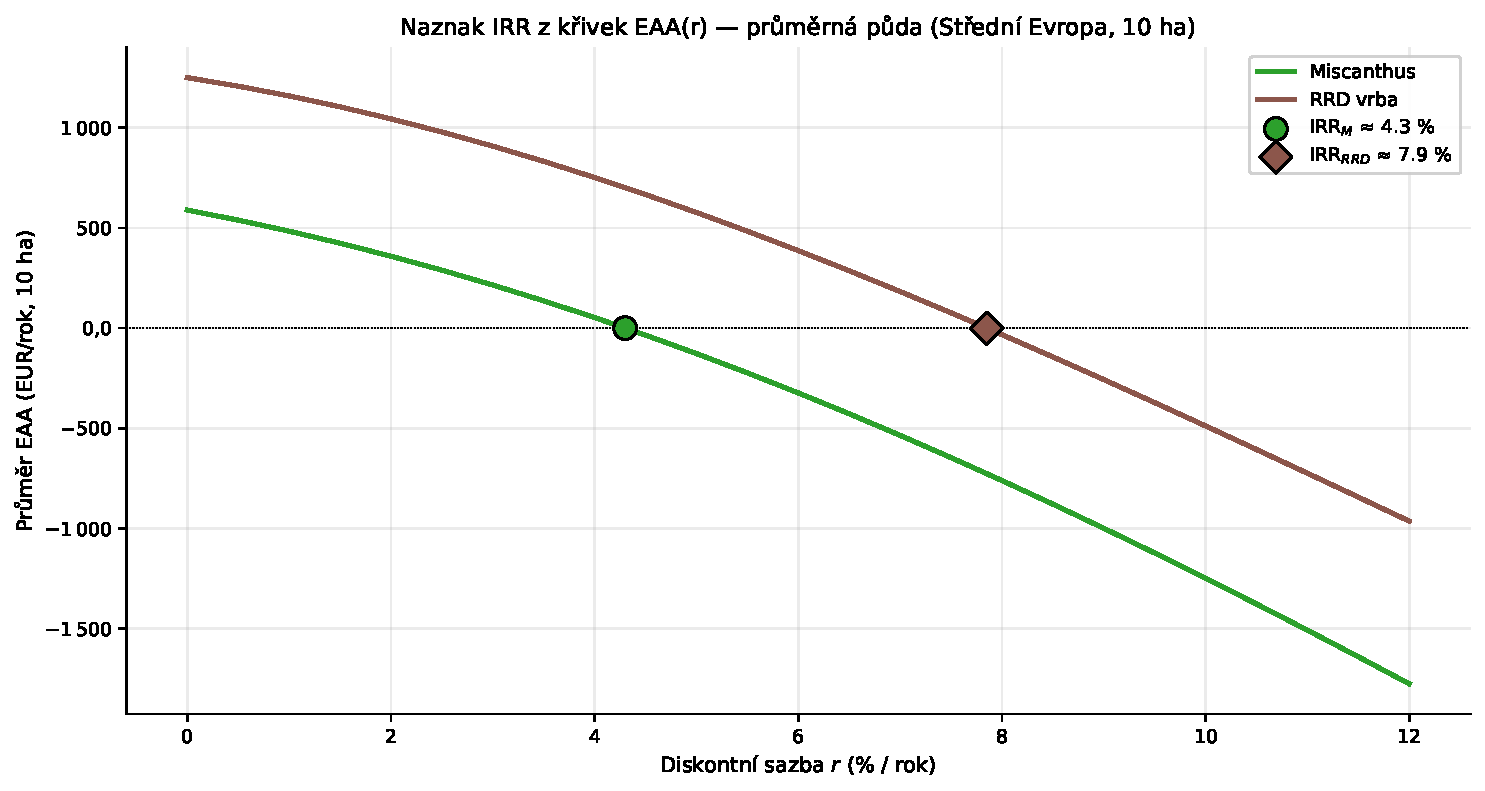
\includegraphics[width=\textwidth]{img/kap04/04_diskont_irr_naznak.pdf}
\caption{Rozdělení vnitřního výnosového procenta (IRR) pro~optimální
půdu, $N = 10\,000$ scénářů. Svislé čáry označují mediány. Tato
distribuce je~kandidátem pro~odvození endogenní diskontní sazby
v~budoucích pracích.}
\label{fig:vysledky-diskont-irr-naznak}
\end{figure}

Z~obrázku a~numerických výstupů plyne pro~optimální půdu:
\begin{itemize}
    \item Miscanthus: medián IRR $14{,}1\,\%$, P25 $11{,}1\,\%$, P75 $17{,}0\,\%$;
    \item SRC vrba: medián IRR $14{,}5\,\%$, P25 $12{,}6\,\%$, P75 $16{,}4\,\%$.
\end{itemize}
Investice je~tedy v~optimálních podmínkách \emph{vysoce výnosná}
($\sim 14\,\%$ ročně) a~SRC vrba má~o~něco užší rozdělení (méně
nejistoty kolem typické výnosnosti). Praktická interpretace pro~rizikově
averzního investora: pokud na~kapitálovém trhu lze získat finance
za~$r < 12\,\%$ (P25 IRR), pak je~projekt na~optimální půdě
ekonomicky atraktivní s~$75\,\%$ jistotou.

\paragraph{Proč tento přístup dává smysl --- a~jeho limity.}
Klasický postup určování diskontu (CAPM, WACC) vyžaduje znalost
beta-koeficientu konkrétního aktiva, market risk premium a~dalších
parametrů kapitálového trhu. Pro~zemědělské energetické plodiny
v~ČR jsou~tato data těžko dostupná a~paralelní studie
\citep{knapek_2024} k~nim přistupuje právě nepřímo (přes srovnání
s~konvenčními plodinami).

Endogenní odvození z~distribuce IRR je~\emph{alternativní cesta},
která~místo dat z~kapitálového trhu využívá výsledky vlastní Monte
Carlo simulace. Její výhody:
\begin{itemize}
    \item Pracuje přímo s~rizikem konkrétního projektu, nikoli
          s~obecným tržním rizikem;
    \item Reflektuje stochastické vlastnosti modelu (počasí, cena, selhání);
    \item Umožňuje investorovi explicitní volbu rizikové tolerance
          (P25 vs.~medián vs.~P75).
\end{itemize}
Nevýhody, které je~třeba v~budoucím výzkumu vyřešit:
\begin{itemize}
    \item Distribuce IRR je~citlivá na~kvalitu půdy --- jiný diskont
          pro~optimální a~průměrnou půdu je~problematický pro~jednotnou
          investiční politiku;
    \item Volba kvantilu (P25, medián, P75) je~stále subjektivní
          a~vyžaduje teoretické zdůvodnění;
    \item Přístup nezahrnuje bezrizikovou sazbu, která~by~měla být
          v~diskontu obsažena podle CAPM principu;
    \item Ignoruje korelaci s~tržním portfoliem (systematické riziko),
          které~je~v~CAPM klíčové.
\end{itemize}
Tyto otevřené otázky představují přirozený směr budoucího bádání.